\chapter{on diversity}
 Morrison et al.\cite{populationDiversity} described the pair-wise Hamming distance as one of the most commonly used measures of distance in genotypic space, and is what will be used here to calculate a populations diversity as one scalar metric. In implementation, this algorithm\ref{eq:Hamming} is counting the number of genomes in all pairs of genotypes which is not identical. Another description is the edit distance between two binary genomes. 


where y is a genotype, P is the population size and L is the number of genomes in a genotype.

A problem with using a pairwise Hamming distance is that the number of computations is quadratic with the size of P. Meaning the computational time is quite long, but since this metric is only to be calculated once when experimentation is completed, the restriction this puts on the experiment is negligible. However, a suggested alternate way of calculating population diversity on the basis of edit distance is by calculating the mean edit distance from every genotype to a \textit{centroid} genotype where the centroid is the average genotype in a population, and its i-th element can be given as  
\begin{equation}
    \label{eq:centroid}
    \varphi_{i}=\tfrac{1}{P}\sum_{j=1}^{P}y_{ji}
\end{equation}
Using this vector that can be calculated linearly with respect to P, a diversity metric \(\Delta\) can be calculated as 
\begin{equation*}
    \Delta = \tfrac{1}{P}\sum_{j=1}^{P}\sum_{i=1}^{L}\left | \varphi_{i}-y_{ji} \right |
\end{equation*}

\begin{equation}
    \label{eq:homemade diversity}
    \Delta = \tfrac{1}{{P}}\sum_{j=1}^{P}\sum_{i=1}^{L}\left | (\tfrac{1}{{P}}\sum_{{j}'=1}^{P}y_{{j}'i})-y_{ji} \right |
\end{equation}
While it is obvious that calculation time grows linearly for larger population sizes and the computational requirements for large experiments are greatly reduced, the pair-wise Hamming distance is a tried and tested diversity metric, and is what will be used to describe the change in diversity between generations and algorithms. 

%%%%%%%%%%%%%%%%%%%%%%%%%%
\begin{equation}
    \label{eq:linearHamming}
    \sum_{j=1}^{j=P-1}\sum_{{j}'=j+1}^{{j}'=P}\sum_{i=1}^{i=L}\left |y_{ij}-y_{i{j}'}\right | = \sum_{i=1}^{L}\left [ \left (  P-\sum_{j=1}^{P}y_{ji} \right )\sum_{j=1}^{P}y_{ji} \right ]
\end{equation}

%%%%%%%%%%%%%%%%%%%%%%%%%%
\begin{figure}
    \label{fig:diversity_comparison}
    \begin{subfigure}[h]{0.49\linewidth}
        \label{fig:diversity_comparison:Hamming}
        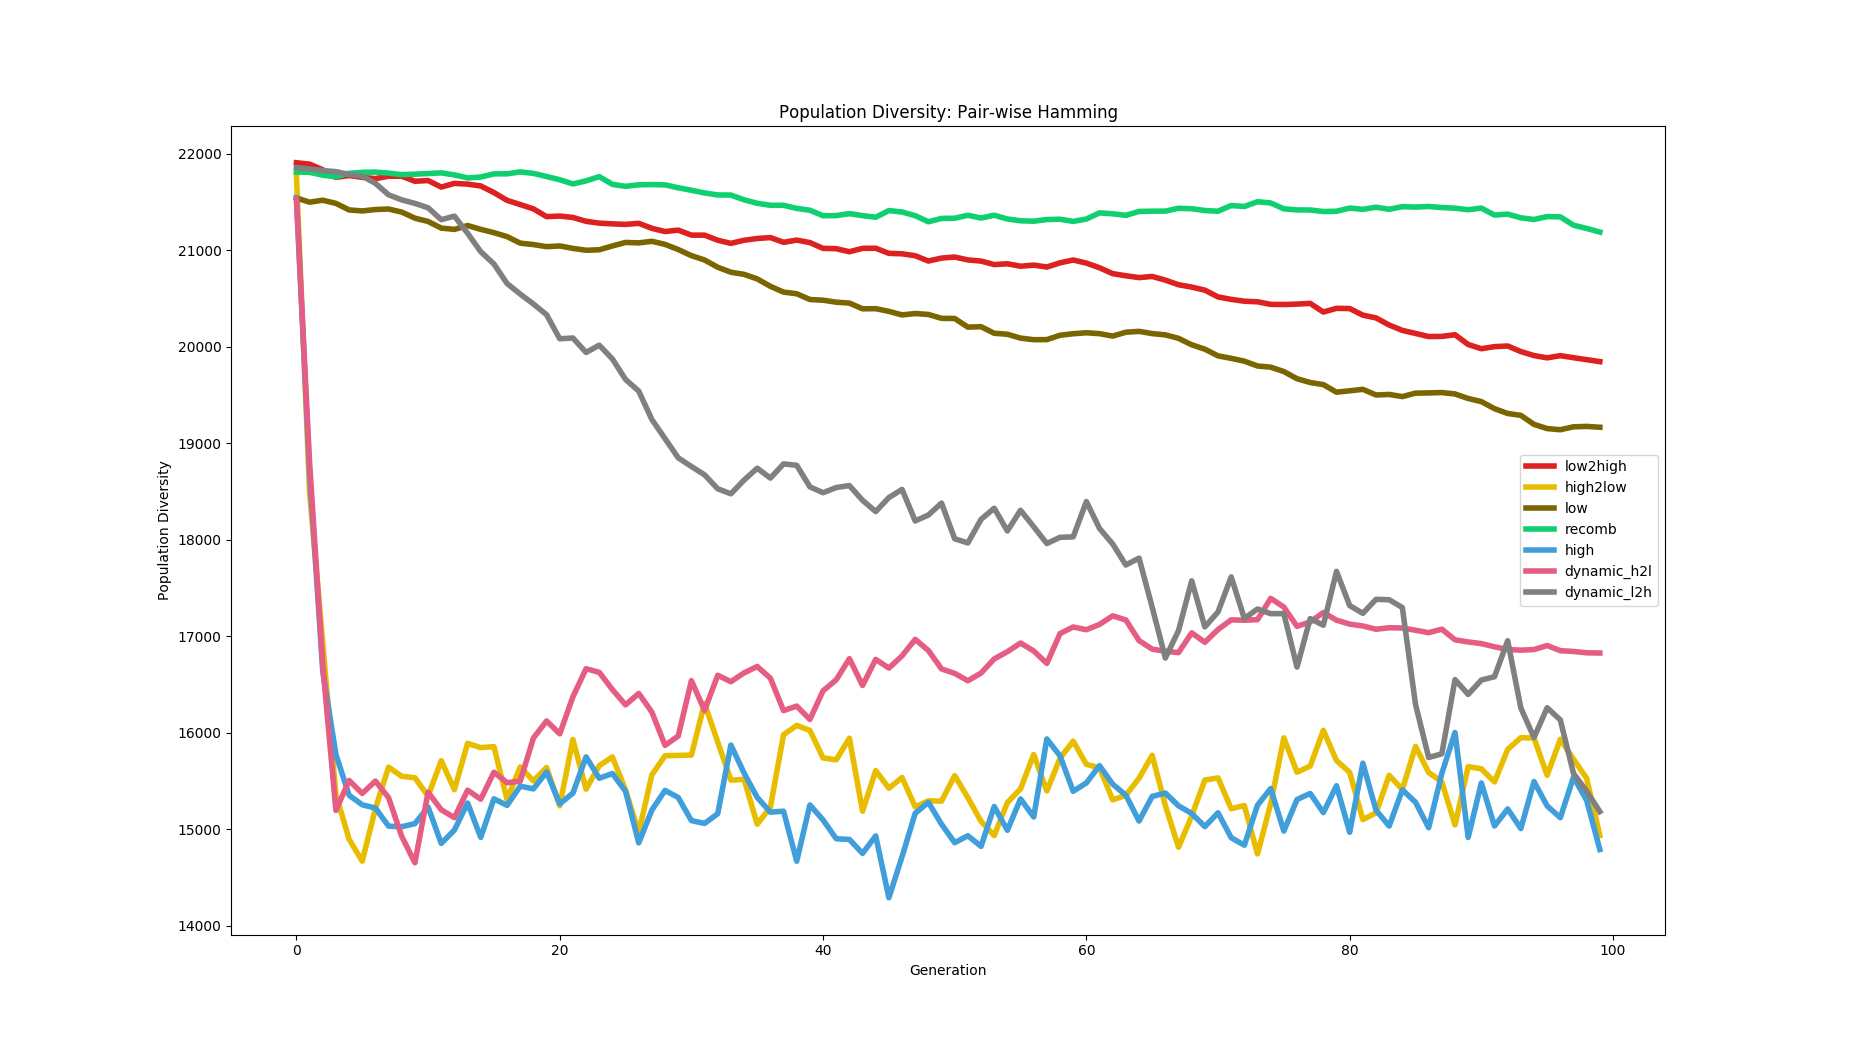
\includegraphics[width=\linewidth]{Chapters/Experiments/search_algo/figures/diversity_showcase_hamming.png}
        \caption{Pair-wise Hamming distance.}
    \end{subfigure}
    \hfill
    \begin{subfigure}[h]{0.49\linewidth}
        \label{fig:diversity_comparison:homemade}
        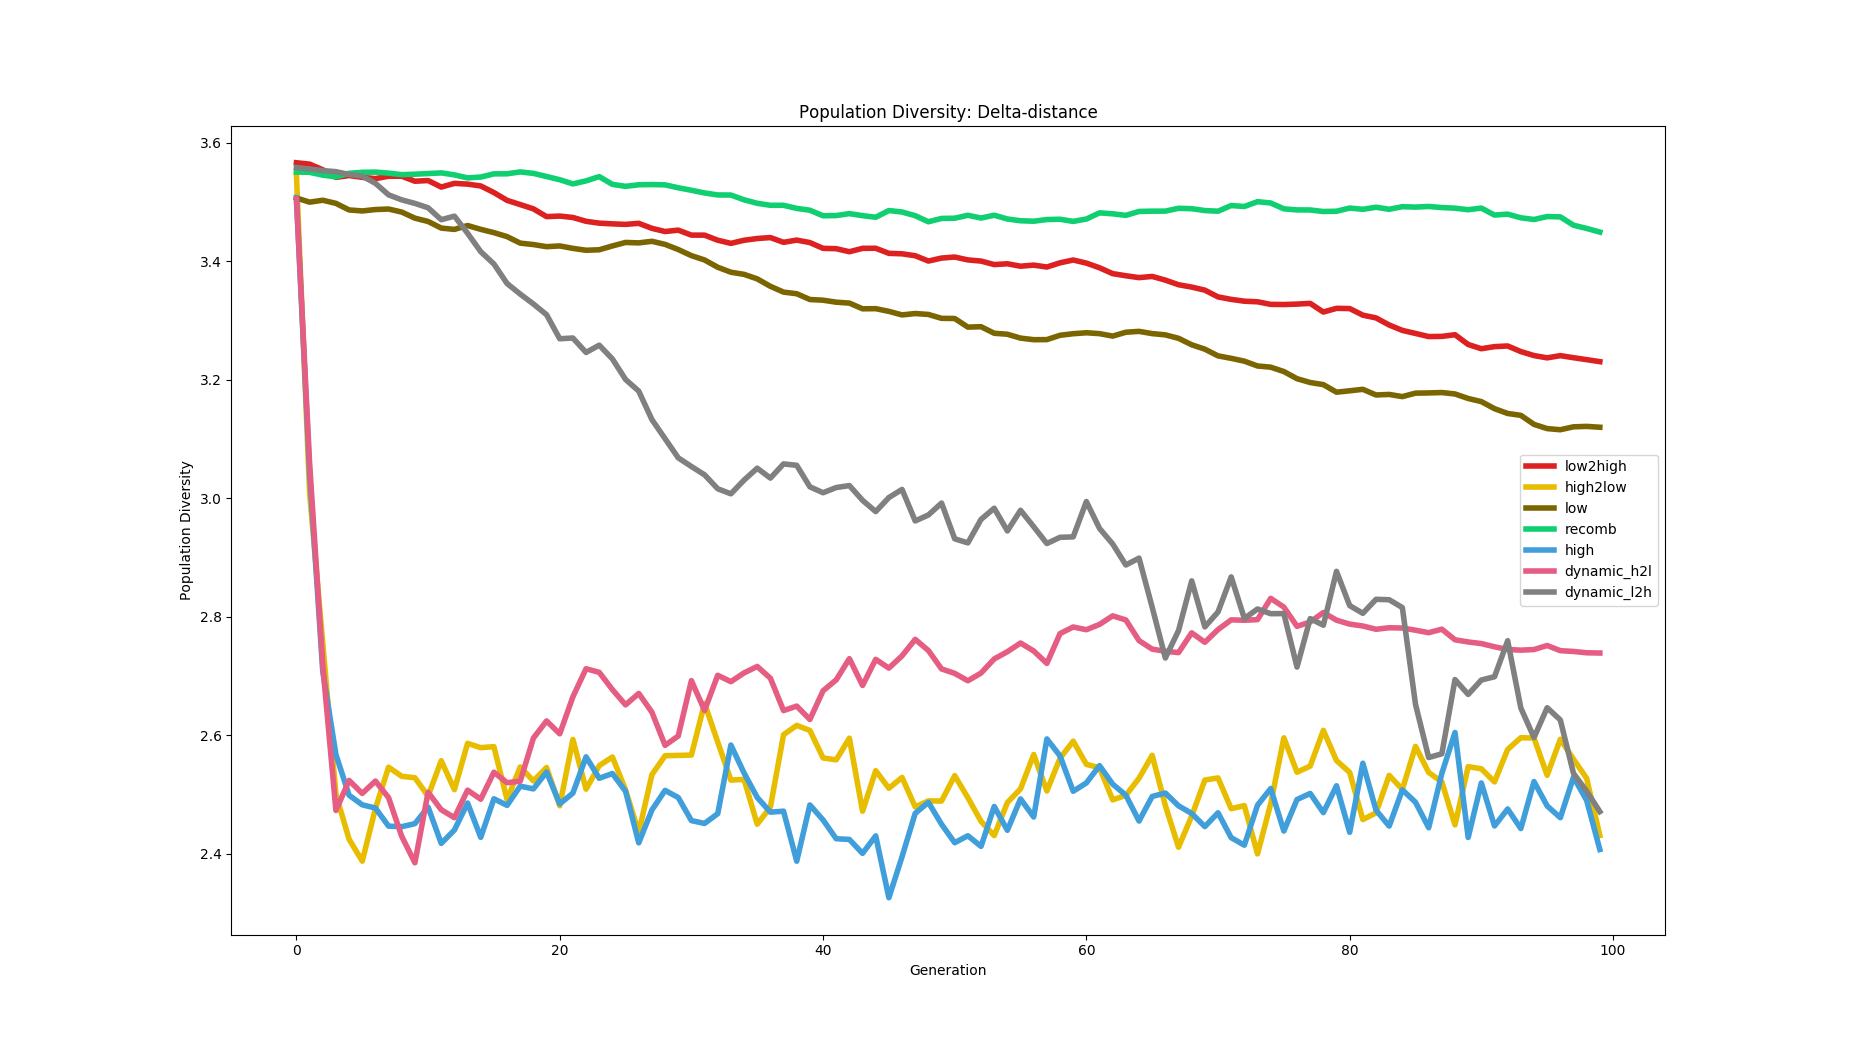
\includegraphics[width=\linewidth]{Chapters/Experiments/search_algo/figures/diversity_showcase_homemade.png}
        \caption{\(\Delta\)-diversity metric}
    \end{subfigure}%
    \caption{A comparison of pair-wise Hamming distance and \(\Delta\)-diversity. The diversity is the average population diversity for each generation during the search for an optimal path for task 1a. Note the similar curves for each algorithm and the scale on the y-axis}
\end{figure}
\chapter{on path size plot}
While algorithms in group 1 and 2 follow their group rule of reaching convergence for high selection pressure, or not converge within 100 generations for the low selection pressures, algorithms 3a and 3b both converge within the 100 first generations. This could be because these searching schemes both are effective ways of optimizing the capacity in paths, or it might be that the average selection pressure within these searches is a selection pressure that works well for this generation limit. We can back up this claim by the fact that algorithms 2a and 2b both converge for task 3 and 4, which for these algorithms and these tasks, have about the same tournament size as the average tournament size in 3a and 3b. 

As a paths size can not change due to mutation, it is reasonable that some of the algorithms with high selection pressure finds optimal sizes which is lower than the average initialized size of 6. This effect could lead to the conclusion that for these tasks, algorithms with high tournament size needs less capacity to solve the task. However, this could be a random effect where some of the initialized paths with fewer modules happened to have a higher fitness. As searches with lower selection pressure all row the average path size or keep it the same, it does not seem that a larger path capacity hurts fitness.
\chapter{}
\chapter{}
- Low trains quickly and reaches a performance the same as most of the other algorithms. Few total number of training iterations cause the modules not to overfit mentionably. A population of 64 and termination limit of 100 might not be well suited for this algorithm though. A higher generation limit would give the algorithm a decent chance at finding a optimal path within its population, and a smaller population size together with maybe a higher mutation rate increase the probability of pretrained(MAYBE JUST A SMALLER PATHNET?) modules to be tried in a path before new modules have optimized so much that introducing a old module to a path would reduce fitness below that of the newly trained modules. - Having a high tournament size for the later searches yield higher module reuse than lower tournament sizes, regardless if the previously trained modules were trained using a high or low tournament size. 
\chapter{Conclusion on reuse: removed because of duplication}
When performing ANOVA tests on the amount of module reuse, a test of the null hypothesis
\begin{equation*}
    H_{0}:\bar{\mu}_{1_{a}}=\bar{\mu}_{1_{b}}=\bar{\mu}_{1_{c}}=\bar{\mu}_{2_{b}}=\bar{\mu}_{3_{a}}
\end{equation*}
yields a P-value not sufficient to reject \(H_{0}\), while adding either 2a or 3b to the test causes \(H_{0}\) to be rejected. While this makes a case for high selection pressure leading to higher reuse, null hypothesis for \(\bar{\mu}_{2_{a}}=\bar{\mu}_{1_{b}}\) can not be rejected, but 2a and 2b is shown to be significantly different from each other. From this, the conclusion drawn is that more experimental runs are needed to be able to say anything meaningful about what causes an increase in module reuse.